\documentclass{report}
\usepackage{pdfpages}
\usepackage[a4paper, top=2cm, bottom=2cm, left=2cm, right=2cm]{geometry}
\usepackage{fancyhdr}
\usepackage{graphicx} 
\usepackage{ulem}
\usepackage{listings}
\usepackage[absolute,overlay]{textpos}
\usepackage{minted}

\lstdefinestyle{cppstyle}{
	language=C++,             % Specify the language
	basicstyle=\ttfamily,     % Set the font to typewriter
	basicstyle=\ttfamily\footnotesize,
	keywordstyle=\color{blue}\bfseries, % Keywords in bold blue
	commentstyle=\color{green},         % Comments in green
	stringstyle=\color{red},            % Strings in red
	numbers=left,            % Line numbers on the left
	numberstyle=\tiny\color{gray}, % Line numbers in tiny gray font
	stepnumber=1,             % Line number step
	breaklines=true,          % Automatic line breaking
	tabsize=4,                % Set tab size
	showstringspaces=false,   % Don't show spaces in strings
	frame=single,             % Add a frame around the code
}

\newcommand{\name}{Marco Söllinger,}
\newcommand{\fach}{SEN2}
\newcommand{\topic}{Übung 1}
\newcommand{\uebungangabe}{Uebung1.pdf}

\newcommand{\matnr}{s2410306011, Gruppe 1}
\newcommand{\uebungsgruppe}{Gruppe 2}
\newcommand{\aufwand}{4}


\pagestyle{fancy}
\normalem 
\fancyhead[R]{Marco Söllinger}  

\begin{document}
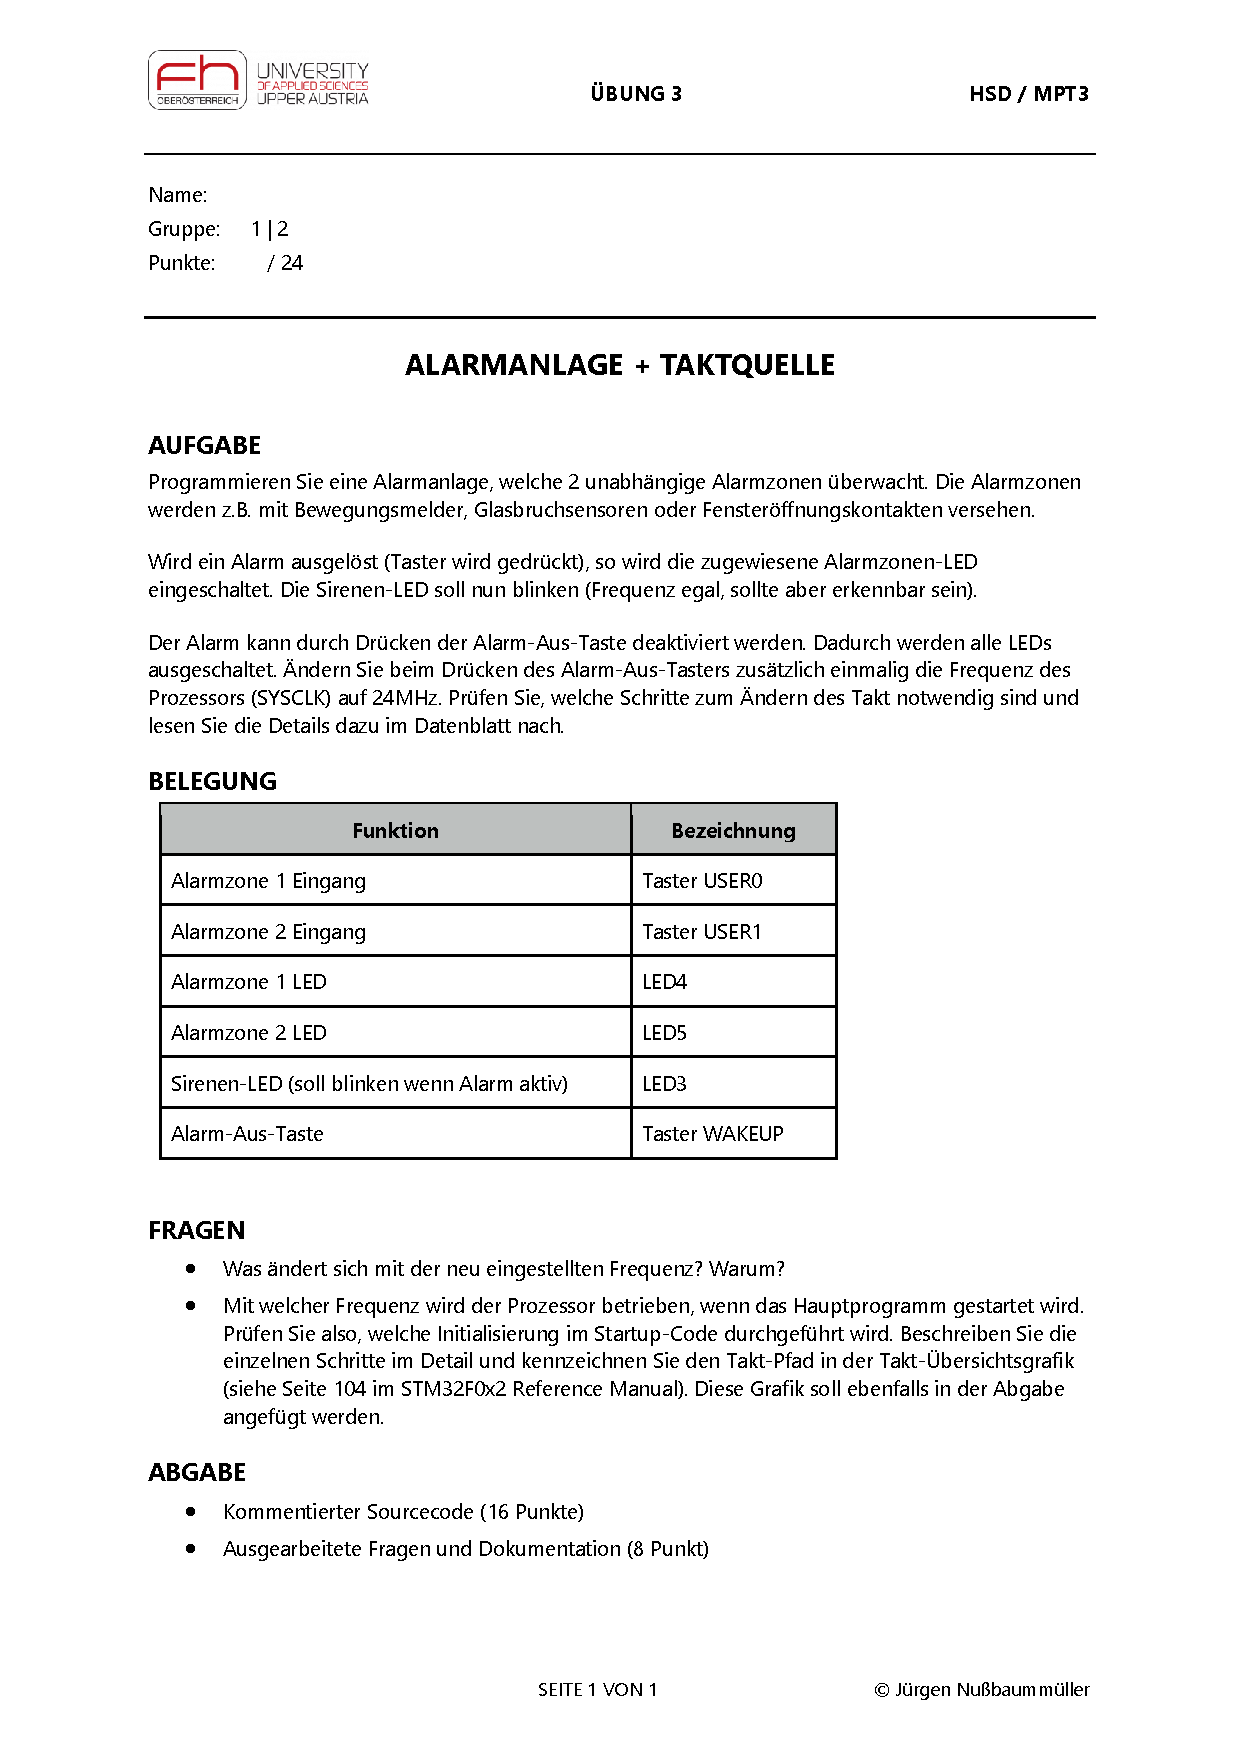
\includepdf[pages=1,pagecommand={
			\begin{textblock*}{10cm}(3.5cm, 3.1cm)
				\textbf{\name}    \textbf{\matnr}
			\end{textblock*}
		}]{./MPT3_Uebung_3.pdf}

\section*{Aufgabe 1:}

\subsection*{1.1 Loesungsidee}
Es wurde die Alarmanlagenlogic in der main.c implementiert.\\
Fuer das periodische Blinken der LED wurden die SysTick verwendet.\\
Fuer das Ansteuern der Peripherie wurde die gegebenen Board Treiber verwendet.\\\\
Fuer das, wechseln der Systemclock Frequenz wurde die Funktion SetSysClock in system\_stm32f0xx.c kopiert und angepasst.\\
Das wechseln zur HSE Clock und ausschalten des PLL wurde noch in die standert SetSysClock Funktion hinzugefuegt.\\
Die neue Implementierung heisst SwitchClockTo24Mhz() und liegt in der main.c Datei.\\
Ausserdem wurde das Aktualisieren der SysTick Zeit in dieser Funktion hinzugefuegt.\\


\subsection*{1.2 Code}
Die Board treiber wurden nicht veraendert und sind in den Board Unterordnern zu finden.\\

\lstinputlisting[style=cppstyle, title=\texttt{main.c} ]{../STM32Base/projects/Alarmanlage/main.c}


\subsection*{1.3 Fragen}
- Was ändert sich mit der neu eingestellten Frequenz? Warum?\\
Wenn man meinen Code ausfuehrt, wie oben gezeigt, aendert das Aufrufen der SwitchClockTo24Mhz Funktion die Systemclock Frequenz von 48Mhz auf 24Mhz.\\
Das Blinken der Led wird dadurch nicht beeinflusst, da die SysTick Zeit ebenfalls angepasst wird mittels:\\
- SystemCoreClockUpdate();\\
- SysTick\_Config(SystemCoreClock / 1000);\\
Diese Aufrufe aktualisieren die SystemTick Zeit auf 1ms bei 24Mhz.\\\\
Wenn diese Aktualisierung nicht gemacht wird, blinkt die LED langsamer, da die SysTick Zeit immer noch auf 1ms bei 48Mhz eingestellt ist.\\\\\\
-  Mit welcher Frequenz wird der Prozessor betrieben, wenn das Hauptprogramm gestartet wird? \\
Wenn der Microcontroller gestartet wird, wird er mit der internen HighSpeed Clock HSI (8Mhz) betrieben. (Hardware default)\\
In der startup.s wird der Reset Handler aufgerufen, welcher die SystemInit Funktion in system\_stm32f0xx.c aufruft.\\
Diese Funktion setzt ein paar Initalzustand und ruft anschliessend die SetSysClock Funktion auf.\\
SetSysClock schaltet den High speed external Clock HSE (8Mhz Quarz) ein, konifiguriert den PLL (8Mhz /1 *6 = 48Mhz), schaltet diese ein und wechselt die Systemclock auf die PLL als source.\\
Ausserdem wird die Flash latency richtig modifiziert, damit der Prozessor bei 48Mhz stabil laeuft.\\
Macht man das nicht, haengt sich der Microcontroller nach einiger Zeit auf.\\\\
\begin{figure}[h!]
	\centering
	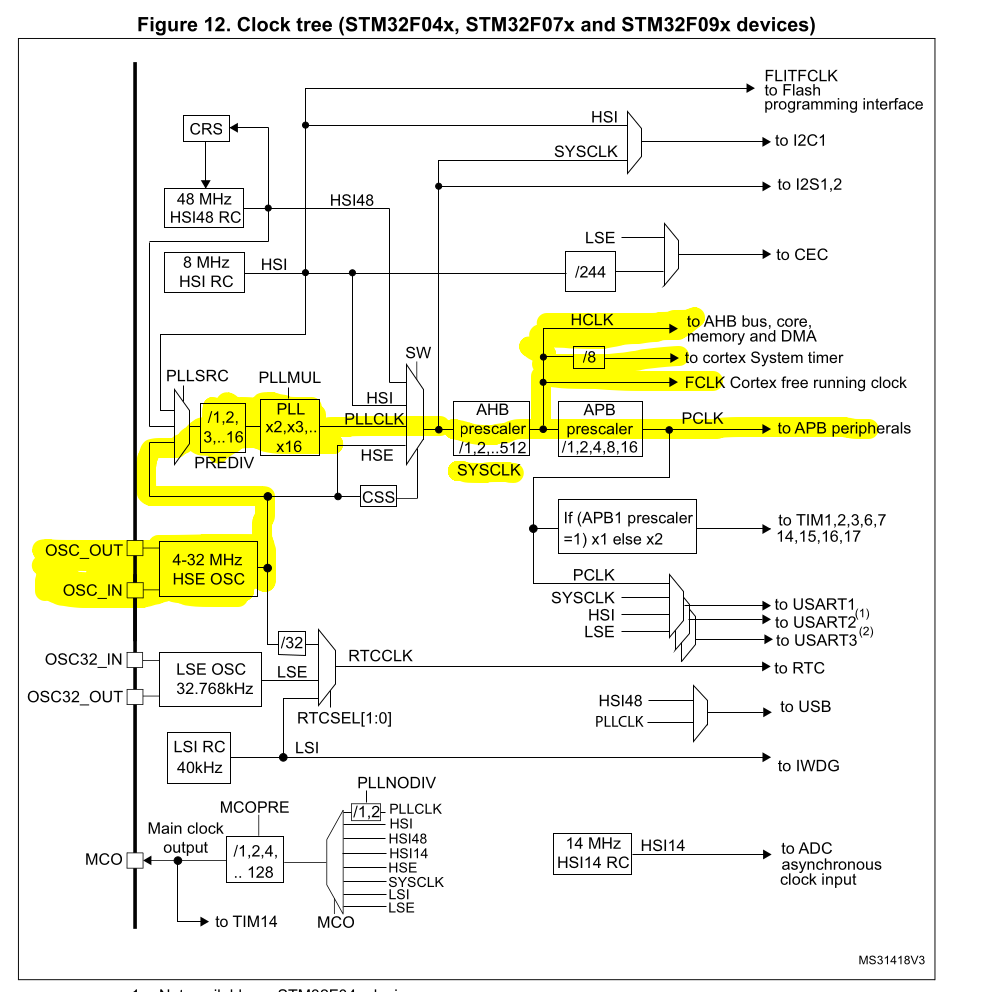
\includegraphics[width=0.6\textwidth]{./Pic.png}
	\caption{Pfad der Sytemclocks}
	\label{Task1_address0x0}
\end{figure}


\end{document}
